%%%%%%%%%%%%%%%%%%%%%%%%%%%%%%%%%%%%%%%%%%%%%%%%%%%%%%%%%%%%%%%%%%%%%%%%%%%%%%%%%%%%%%%%%%%%%%%%%%%
% Chapter 2 -> Background
% Author: Mingbo Cheng
%%%%%%%%%%%%%%%%%%%%%%%%%%%%%%%%%%%%%%%%%%%%%%%%%%%%%%%%%%%%%%%%%%%%%%%%%%%%%%%%%%%%%%%%%%%%%%%%%%%
\chapter{Background}
\label{cha:background}
\graphicspath{{chapter2/figs/}}

In this chapter, we introduce the background knowledge needed to understand the thesis including biology and computational aspects. First, we talk about the molecular biology(Section 2.1). Next, we introduce the advances of single cell sequencing technologies(Section 2.2) including single cell transcriptome profiling, open chromatin measurements and protein profilling in single cell. In this section, we also describe sequncing protocols that simultaneously measure more than one type of features, i.e. multimodal sequencing. Next, we introduce the computational to analyze different single cell technologies assays, and also common workflow of mulitmodal analysis. Next, we describe current state-of-the-art methods for multimodal integration and trajectory inference(Section 2.3). Last 


\section{DNA Organization, chromatin accessibility and gene regulation}
In the symphony of life, the function of DNA organization, chromatin accessibility, and gene regulation orchestrates a harmonious dance that dictates the fate and functioning of every living organism. We start this section by first introducing DNA organization. Next, we talk about chromatin accessibility followed by the introduction of gene regulation.

Deoxyribonucleic Acid, or DNA is the genetic blueprint of life, containing the instructions for the development and functioning of living organisms. It is a long, double-stranded helical structure composed of four nucleotide building blocks: adenine (A), thymine (T), cytosine (C), and guanine (G). The sequence of these nucleotides forms the genetic code, encoding instructions for the development, functioning, and maintenance of all living organisms. DNA is organized into structures called chromosomes, which are located in the cell nucleus.


\begin{figure}[!ht]
	\centering
	\includegraphics[width=0.95\textwidth]{chromatin_organization/fig}
	\vspace{0.1cm}
	\caption[chomosome, chromatin and gene regulation.]{The figure illustrates the the how gene regulation processed. \emph{Source: ~\citep{heumos2023best}}(modified to fit thesis format and/or clarify key points)}
	\label{fig:chromatin_organization}
\end{figure}


Chromatin is the complex of DNA and proteins found in the nucleus of a cell. Chromatin accessibility is a crucial molecular concept that describes the degree to which DNA is available or accessible for cellular processes, particularly gene expression. It can exist in two states: open and condensed. Open chromatin refers to the relaxed, accessible state where DNA is available for transcription and gene expression. In this state, the DNA is not tightly wound around histone proteins, allowing regulatory proteins and RNA polymerase to easily access specific DNA sequences, facilitating the transcription of genes into RNA. Open chromatin is associated with active gene expression and is influenced by various factors, including epigenetic modifications such as acetylation and methylation. Conversely, in a "closed" or condensed chromatin state, the DNA is tightly wound around histone proteins, making it less accessible. This state inhibits the binding of transcriptional machinery, leading to reduced or suppressed gene expression. Closed chromatin is associated with inactive or silenced genes.

Gene regulation refers to the mechanisms that control the expression of genes. While an organism's DNA carries the instructions for a vast array of biological processes, not all genes are active all the time. Gene regulation allows cells to turn genes on or off, and to fine-tune their activity. This regulation is achieved through the interaction of regulatory proteins, transcription factors, and other molecules that bind to specific DNA sequences, influencing the initiation or inhibition of transcription. Epigenetic modifications, such as DNA methylation and histone modification, also play a crucial role in gene regulation by modifying the accessibility of DNA.


\section{Single cell sequencing technology}
Since Sanger sequencing~\citep{sanger1975rapid} analysis was introduced in 1975, numerous advances in methodology have been developed to improve the understanding of the heterogeneity and transcriptomic states present in complex biological systems. The invention of a series of rapidly evolving Next Generation Sequencing (NGS) technologies revolutionarily facilitates the study of heterogeneous biological processes with high throughput, shorter time and lower cost. NGS enables researchers to perform profiling of epigenomes, transcriptomes and proteomes. The development of single-cell sequencing technology further enables the study of heterogeneity at single-cell resolution. In this section, we will briefly introduce single-cell sequencing technology, single-cell RNA sequencing, single-cell ATAC sequencing and single-cell protein sequencing.


\begin{figure}[!ht]
	\centering
	\includegraphics[width=0.95\textwidth]{multimodal-single-cell/fig}
	\vspace{0.1cm}
	\caption[open chromatin, transcriptome, and surface protein profiling in a single celll.]{multimodal singel cell. \emph{Source: ~\citep{zhu2020single}}(modified to fit thesis format and/or clarify key points)}
	\label{fig:multimodal_single_cell}
\end{figure}



\subsection{Transcriptomics profiling with scRNA-seq}

\begin{figure}[!ht]
	\centering
	\includegraphics[width=0.95\textwidth]{rna_scRNA/fig}
	\vspace{0.1cm}
	\caption[bulk rna and single cell rna sequencing comparison.]{bulk rna and single cell rna sequencing.}
	\label{fig:rna_scRNA}
\end{figure}

Single-cell RNA sequencing (scRNA-seq)\citep{singlecellsequencing2014, singlecellsequencing2015} has emerged as a powerful tool that allows the study of gene expression at the individual cell level, providing insights into the heterogeneity and dynamics of cellular responses in various biological contexts. In contrast to traditional bulk RNA-seq, which averages gene expression across millions of cells, scRNA-seq enables the investigation of transcriptomic profiles within specific cell types, offering a more detailed understanding of cellular behaviors during development or in response to perturbations.

Single-cell RNA sequencing(scRNA-seq) was introduced in 2009 ~\citep{tang2009mrna}. In general, scRNA-seq protocols can be classified into droplet-based and plate-based methods. Droplet-based methods use droplet microfluidics technology~\citep{dropletcompare2019, droplet2019practice} to capture cells in each droplet. In this procedure, a dissociated mixture of cells is introduced into a microfluidic device, while beads coated with primers are introduced at a separate input. The device is specifically designed to create aqueous droplets within mineral oil, with the inputs strategically arranged to enable the simultaneous capture of cells and beads within a droplet. In this capture event, the reagents carried along with the bead induce cell lysis, allowing poly(A) tagged RNA molecules to bind to the capture probes on the bead's surface. Subsequently, reverse transcription and PCR amplification are initiated, resulting in the generation of an individual cDNA library for each cell, which is uniquely tagged with the barcode sequence present on the bead. A variety of droplet-based methods have beend developed including Drop-seq~\citep{dropseq2015}, inDrop~\citep{indrop2015} and GemCode/Chromium 10X~\citep{zheng2017massively}. Droplet-based capture technologies offer the advantage of capturing a significantly larger number of cells simultaneously, reaching up to tens of thousands. Additionally, these approaches exhibit reduced selectivity regarding cell size and generate fewer doublets. Plate-based methods employ passive cell separation into discrete wells on a plate. In these wells, cells undergo processes such as lysis, reverse transcription, and subsequent PCR amplification of the gathered cDNA. Following these steps, the resulting product is extracted from the plate, and libraries are then prepared for Illumina sequencing. Many plate-based methods have been developed including CEL-Seq\citep{hashimshony2012celseq}, CEL-Seq2\citep{hashimshony2016celseq2}, SMART-seq~\citep{goetz2012smartseq} and SMART-seq2~\citep{Picelli2014smartseq}. Plate-based cell capture technologies utilize chips with a fixed-size window, limiting the capture to cells of specific sizes during a single run. Droplet-based techniques are currently the most commonly used cell capture technologies in single-cell RNA fields, whereas plate-based methods are more expensive and time-consuming.

Droplet-based capture methods often incorporate Unique Molecular Identifiers (UMIs), and short random nucleotide sequences. Given the minimal RNA amounts in individual cells (approximately 10-30 pg, with less than 5 percent being mRNA), a crucial PCR amplification step is employed to generate sufficient cDNA for sequencing. Variable amplification rates based on nucleotide sequences can introduce distortions in transcript proportions within a library. UMIs aim to improve gene expression quantification by aiding in PCR duplicate removal during amplification In droplet-based capture protocols, nucleotide probes include a poly(T) sequence binding to mature mRNA, a consistent barcode sequence across all probes on a bead, and an 8-10 base UMI sequence unique to each probe. The length of UMI sequences makes capturing two copies of a transcript on two probes with the same UMI highly improbable. After reverse transcription, amplification, sequencing, and alignment, de-duplication involves identifying reads with the same UMI aligning to the same position, indicating PCR duplicates rather than genuinely expressed transcript copies. To ensure method effectiveness, each read must be associated with a UMI, resulting in sequencing only a small section at the 3' end of each transcript. 


\subsection{Chromatin accessibility profiling with scATAC-seq}

Advancements in Next-Generation Sequencing (NGS) technology have led to the development of various methods for comprehensive genome-wide profiling of chromatin accessibility through sequencing. DNase-seq(deoxyribonuclease I hypersensitive sites sequencing)\citep{boyle2008dnasseq} uses DNase I nuclease to perform the digestion. FAIRE-seq(formaldehyde-assisted isolation of regulatory elements sequencing)\citep{giresi2007faireseq} physical isolation of protein-bound and protein-free DNA fragments. ATAC-seq(assay for transposase-accessible chromatin using sequencing)\citep{buenrostro2013atacseq} use Tn5 transposase to insert sequencing adapters into accessible regions of the genome. Due to the employment of a hyperactive Tn5 transposase, which tags and fragments DNA sequences in open chromatin regions simultaneously, ATAC-seq requires shorter sample preparation times and a lower number of cells for high-quality profiling of chromatin accessibility compared to other methods, ATAC-seq has gained prominence as the most extensively utilized.\citep{minnoye2021chromatin}.

Protocols for single-cell ATAC-sequencing (scATAC-seq) have been devised, enabling the unbiased identification of cell-type-specific regulatory elements within heterogeneous cell populations. This approach boasts a high throughput, capable of processing tens of thousands of cells per assay. scATAC-seq has proven successful in elucidating the regulatory landscape of adult mouse tissues \citep{cusanovich2018single}, as well as in studying the human and mouse brain \cite{lake2018humanbrain, sinnamon2019accessible} etc. Several scATAC-seq methods have been developed to measure open chromatin at single cell level, e.g., the Microfluidics-based method (Buenrostro et al., 2015), which uses physical isolation of single cells. Specifically, it employs a programmable microfluidics device to compartmentalize single cells into nanoscale reaction chambers. After cell viability is confirmed with the use of a microscope, ATAC-seq is performed on each captured cell individually. sci-ATAC-seq(the split-and-pool combinatorial cellular indexing) method \citep{cusanovich2015multiplex} performs several rounds of combinatorial indexing to uniquely barcode individual cells. First, it uses a cell sorter to dispense a defined number of nuclei (typically 2,500) into the wells of a 96-well plate, each containing a Tn5 transposase loaded with a unique combination of barcodes. The tagmentation reaction thus introduces the first round of indexes. Next, the nuclei are pooled, mixed and dispensed in each well of 96-well plates in the defined number of 25 nuclei. Each well contains a unique combination of barcoded adaptors, which are integrated during the PCR amplification thus providing the second round of indexing. After sequencing, it is then possible to identify each cell 26 based on a unique set of barcodes. Due to the number of nuclei aliquoted in each well for the second indexing round at least 100 times lower than the first indexing round, the number of collisions, namely, cells having identical barcodes is statistically ensured to be low (estimated and measured at ~ 11\%). Another highly effective method is the droplet-based single-cell Assay for Transposase-Accessible Chromatin with sequencing (scATAC-seq)\citep{satpathy2019massively}, involving cell partitioning through a microfluidic device. Initially, nuclei are isolated from a single-cell suspension and transposed in bulk using transposase Tn5. Subsequently, transposed nuclei are loaded onto a microfluidic chip to generate gel beads in emulsion (GEM). Each gel bead is barcoded with single-stranded oligonucleotides, comprising a 29-bp sequencing adapter, a 16-bp barcode selected from 750,000 designed sequences for GEM indexing, and the first 14 bp of read 1N, serving as the priming sequence in the linear amplification reaction for barcode incorporation into transposed DNA. After GEM generation, gel beads are dissolved, releasing oligonucleotides for linear amplification of transposed DNA. Finally, the droplet emulsion is broken, and barcoded DNA fragments are pooled for PCR amplification, generating indexed libraries suitable for high-throughput sequencing. Due to the advantages of high throughput and low costs for droplet-based single-cell ATAC-seq technology, the method is increasingly popular and has been commercialized by 10x Genomic(Chromium Next Gem Single Cell ATAC-seq Library Kit)\cite{satpathy2019massively}.


%\subsection{Protein profiling in single cell}
%%Protein analysis at the single-cell level has relied on the use of antibodies that bind specifically to target proteins. Flow cytometry uses fluorescently labeled antibodies to convert protein signals into fluorescence signals~\citep{@article{kim2022single}
%Secreted proteins play crucial roles in facilitating diverse biological processes, including cell–cell communication, differentiation, migration, and maintaining homeostasis at the population or tissue level. Methods for directly measuring specific protein-secreting cells in clinical settings include enzyme-linked immunospot (ELISPOT) and its variants, such as fluorescence-based immunospot (FluoroSpot) ~\citep{perfetto2004seventeen, karlsson2003comparison}. Indirect assessment of protein secretion function can be conducted through intracellular staining using fluorescence-activated cell sorting (FACS)~\citep{bonner1972fluorescence}. The detection of multiple cytokines in single cells has become possible through intracellular cytokine staining using multicolor flow cytometry ~\citep{irish2004single,hale2009stage}. Mass cytometry is a deviation from traditional flow cytometry utilizing mass spectrometry for detection via rare earth metal probes, has demonstrated highly multiplexed measurement of surface and intracellular proteins~\citep{spitzer2016mass}.
%

\begin{figure}[!ht]
	\centering
	\includegraphics[width=0.95\textwidth]{scATAC-seq/fig}
	\vspace{0.1cm}
	\caption[ATAC sequenceing schematic flow.]{ATAC sequencing. \emph{Source: ~\cite{yan2020reads}} (modified to fit thesis format and/or clarify key points)}
	\label{fig:ATAC-seq}
\end{figure}



\begin{figure}[!ht]
	\centering
	\includegraphics[width=0.95\textwidth]{multi-model-methods/fig}
	\vspace{0.1cm}
	\caption[multimodal methods protocols for Transcriptome, Genome, EpiGenome and Proteome]{multimodal methods protocols for Transcriptome, Genome, EpiGenome and Proteome. \emph{Source: ~\cite{lee2020single}} (modified to fit thesis format and/or clarify key points)}
	\label{fig:piechart-mulitmodal-methods}
\end{figure}



\subsection{Simultaneous multi-modal profiling of single cell}
Single-cell multi-modal technologies typically analyze various types of molecules within a single cell, providing a more profound understanding of biology compared to studying individual molecular layers from separate cells. These advanced technologies unveil cellular heterogeneity across multiple molecular levels within a cell population, offering insights into the interconnectedness or independence of variation across different modalities. The datasets produced by these techniques hold the potential to facilitate a more comprehensive comprehension of the fundamental biological processes and mechanisms that contribute to cellular heterogeneity. Furthermore, they shed light on the associations between normal development, aging, disease etiology, and the intricate links between these phenomena. A variety of multi-modal profiling methods have been proposed recently, see figure Table.\ref{tab:multimodal-methods}

\begin{table}[!ht]
	\footnotesize
	\centering
	\begin{tabular}{lll}%{0.1\linewidth}}
		\toprule
		{\textbf{Modalities}}  & {\textbf{Protocols}} & {\textbf{reference}} \\ 
		\midrule
		\multirow{5}{*}{\shortstack[l]{\includegraphics[scale=1]{multi-model-methods/Protein_RNA.pdf}}}
		   & PLAYR & {~\cite{frei2016playr}} \\
		   & CITE-seq & {~\cite{stoeckius2017citeseq}} \\
           & REAP-seq & {~\cite{peterson2017reapseq}}\\
           & RAID & {~\cite{Gerlach2019RAID}} \\
		   & ECCITE-seq & {~\cite{mimitou2019ECCITE}}\\
		\midrule
		\multirow{5}{*}{\shortstack[l]{\includegraphics[scale=1]{multi-model-methods/RNA_ATAC.pdf}}}
		   & sci-CAR & {~\cite{cao2018scicar}}\\
           & SNARE-seq & {~\cite{chen2019SNARE}} \\
           & scNMT-seq & {~\cite{clark2018scnmt}}\\
		   & scCAT-seq & {~\cite{liu2019scCAT}} \\ 
           & multiome & ~10x Genomics\\
		\midrule
		\multirow{5}{*}{\shortstack[l]{\includegraphics[scale=1]{multi-model-methods/3.pdf}}}
		& TEA-seq & {~\cite{swanson2021simultaneous}}\\
		& DOGMA-seq & ~\cite{mimitou2021scalable} \\
		\\
		\\
		\\
		\bottomrule
	\end{tabular}
	\vspace{0.1cm}
	\caption[Major multimodal methods]{major multimodal methods.}
	\label{tab:multimodal-methods}
\end{table}

\begin{figure}[!ht]
	\centering
	\includegraphics[width=0.95\textwidth]{droplets_multiome_scRNA_scATAC/fig}
	\vspace{0.1cm}
	\caption[10X Droplets-based simultaneous sequencing of scRNA and scATAC.]{droplets\_multiome\_scRNA\_scATAC. \emph{Source: ~\cite{satpathy2019massively}} (modified to fit thesis format and/or clarify key points)}
	\label{fig:droplets_multiome_scRNA_scATAC}
\end{figure}


\section{Computational analysis of single cell}
\subsection{alignment}
The first step in the computational analysis of ATAC-seq/RNA-seq/Protein-seq is the alignment. We input raw sequencing reads and produce an alignment file that contains all mapped DNA reads by aligning them to the reference genome. The objective of alignment is to identify the most probable position of these reads given a vast reference genome with billions of base pairs. The most widely used ATAT-seq alignment tool is Bowtie2 whereas the most popular that for RNA-seq is STAR. These tools are utilized in the Cell Ranger ATAC/RNA/ARC pipeline developed by 10$\times$ Genomics. See Fig. \ref{fig:aligment}
\subsection{scRNA}
We here describe the computational workflow for scRNA-seq data analysis, including preprocessing(quality control, normalization, feature selection), core analysis (dimensionality reduction, batch correction and clustering), and downstream analysis (cell annotation, trajectory analysis, geneset enrichment and ).
\begin{figure}[!ht]
	\centering
	\includegraphics[width=0.95\textwidth]{alignment/fig}
	\vspace{0.1cm}
	\caption[DNA fragments alignment schematic.]{ Illustration of the mapping process. The input consists of a set of reads and a reference genome. In the middle, it gives the results of mapping: the locations of the reads on the reference genome. The first read is aligned at position 100 and the alignment has two mismatches. The second read is aligned at position 114. It is a local alignment with clippings on the left and right. The third read is aligned at position 123. It consists of a 2-base insertion and a 1-base deletion. \emph{Source: ~\cite{galaxyprojectSequenceAnalysis2016alignment}} (modified to fit thesis format and/or clarify key points)}
	\label{fig:alignment}
\end{figure}


\begin{figure}[!ht]
	\centering
	\includegraphics[width=0.95\textwidth]{workflow_scRNA/fig}
	\vspace{0.1cm}
	\caption[A common computational scRNA analysis workflow]{workflow scRNA. \emph{Source: ~\cite{heumos2023best}} (modified to fit thesis format and/or clarify key points)}
	\label{fig:workflow_scRNA}
\end{figure}

\subsubsection{pre-processing}
We start from a count matrix where the mRNA sequence reads obtained are aligned to genes and cells of origin through an alignment pipeline e.g 10$\times$ cellranger pipeline. The pipeline utilizes either cellular barcodes or unique molecular identifiers (UMIs) in conjunction with a reference genome. We eventually obtain a count matrix representing cells by genes. 
\begin{description}
	\item[quality control] We focus on droplet-based scRNA data quality control. Fig~\ref{fig:QCcells}A shows an intact droplet, where a droplet includes a cell and barcode bead to mark the cell ID. The objective of quality control is to filter low-quality droplets like Fig~\ref{fig:QCcells}BCDE and correct the noise. Cells characterized by a low number of detected genes, a shallow count depth, and a high proportion of mitochondrial counts are commonly referred to as low-quality cells. This designation is often indicative of cells in a state of decline, potentially exhibiting compromised membranes associated with cell damage or death. Low-quality cells are detected and filtered either by manually setting thresholds, as suggested in a guide ~\citep{luecken2019current}, or through sample-wise automatic filtering based on the number of median absolute deviations~\citep{germain2020pipecomp}. A variety of methods have been proposed for doublets detection such as DoubletFinder, Scrublet and DoubletDecon\citep{mcginnis2019doubletfinder, wolock2019scrublet, depasquale2019doubletdecon}.
	\item[normalization]  Cells may exhibit varying numbers of gene counts due to disparities in cell size or random variations during sequencing. Count normalization is employed to ensure comparability in cellular profiles. The following variance stabilization ensures that outlier profiles have a limited impact on the overall data structure. A common normalization method involves dividing the raw UMI count by the total detected RNAs in each cell, multiplying the result by a scaling factor (typically set at 10,000), adding a pseudo-count (usually 1), and subsequently applying a log transformation to the outcome. This size-factor normalization effectively mitigates technical variations arising from sequencing depth, while the log transformation serves to alleviate the impact of expression outliers. This approach is particularly valuable in preventing high-abundance genes from disproportionately influencing downstream analyses due to their elevated technical variability. Log-normalization is the default method in the most popular single cell analysis toolkit Seurat~\citep{stuart2019seurat3} written in R and scanpy\citep{wolf2018scanpy} implemented in python. Other methods like scran, sctransform~\citep{l2016scran,hafemeister2019sctransform} are also being used to normalize the count matrix in some scenarios. 
	\item[feature selection] Single-cell RNA-seq datasets typically contain more than 20,000 genes. Numerous genes lack informativeness and predominantly consist of zero counts. Thus, feature selection is necessary to select the most informative features(usually 3,000~5,000 genes) and reduce the computing resources. The objective is to exclude uninformative genes that may not reflect meaningful biological variation across samples. Of all these feature selection approaches, Seurat categorizes genes based on their average expression, and the gene presenting the greatest ratio of variance to mean within each group is chosen as the Highly Variable Gene (HVG) for that particular bin. ~\citep{stuart2019seurat3}; SCMarker selects features without the need for label information, which assesses the number of modalities for each gene through its expression profile~\citep{wang2019scmarker}; M3Drop models the relationship between mean expression and dropout rate~\citep{andrews2019m3drop}; And OGFSC, a variant of HVGs, based on modeling coefficient of variance of genes across cells. ~\citep{hao2019OGFSC}
\end{description}

\begin{figure}[!ht]
	\centering
	\includegraphics[width=0.95\textwidth]{QC_cells/fig}
	\vspace{0.1cm}
	\caption[Droplets-based sequencing of dying cells, doublet and empty droplet .]{QC cells. \emph{Source: ~\cite{heumos2023best}} (modified to fit thesis format and/or clarify key points)}
	\label{fig:QCcells}
\end{figure}
\subsubsection{Dimensional reduction and Clustering}
\begin{description}
	\item[dimensional reduction] Dimensional reduction is twofold: to retain the distances between cells and to visualize the data. scRNA usually uses Principal Component Analysis (PCA) to reduce the dimensionality of the data and retain the distances between cells. While Uniform Manifold Approximation and Projection (UMAP) or t-Distributed Stochastic Neighbor Embedding (t-SNE) are commonly used to visualize the data~\citep{mcinnes2018umap, van2008tsne}.
	\item[batch correction] Batch effects are a common confounding factor in single-cell RNA-seq experiments. Batch effects are systematic differences in measurements between batches (e.g., technical replicates, different days of lab work, different individuals, etc.) that are not due to the biological signal of interest. Batch effects can be caused by a variety of factors, including differences in reagents, equipment, and personnel. Many methods have been proposed to correct batch effects. Seurat uses canonical correlation analysis (CCA)~\citep{stuart2019seurat3} to find anchors between batches and then uses the anchors to do the correction. Scanpy uses batch-balanced k-nearest neighbors (BBKNN)~\citep{polanski2020bbknn} to find mutual nearest neighbors between batches to correct batch effects. Harmony~\citep{korsunsky2019harmony} iteratively removes batch effects present by clustering similar cells from different batches at each iteration while maximizing the diversity of batches within each cluster and then calculates a correction factor for each cell to be applied. Benchmarking of batch correction methods~\citep{tran2020benchmarking} shows that Harmony is the best method.
	\item[clustering] With the batch-corrected data, we next can cluster cells into groups with similar expression profiles that explain the heterogeneity in the data. Many methods have been proposed for clustering, and graph-based clustering methods are the most popular. E.g. Seurat uses Louvain as the default clustering algorithm~\citep{stuart2019seurat3} whereas Scanpy sets default clustering methods with Leiden algorithm~\citep{traag2019louvain}. An independent benchmarking of clustering methods ~\citep{duo2018benchclustering} shows SC3~\citep{kiselev2017sc3} and Seurat delivered the overall best performance and were the only ones to properly recover the cell types in the droplet-based data sets.
	\item[reference mapping] With an existing similar annotated single cell reference data, reference mapping is to transfer labels from the annotated data to the new studies. Seurat uses Canonical Correlation Analysis (CCA) to find anchors between the new dataset and the reference dataset and then transfer labels from the reference dataset to the new dataset. scArches~\citep{lotfollahi2022scarches} reuses neural network models by adding input nodes and weights for new studies and then fine-tuning only those parameters using a neural network to transfer labels from the reference dataset to the new dataset. Symphony builds upon Harmony~\citep{korsunsky2019harmony} batch correction method which can also query the position of a cell in the reference embedding ~\citep{kang2021symphony}.  
\end{description}

\subsubsection{Downstream analysis}
\begin{description}
	\item[Differential gene expression] Differential gene expression is to find which genes are significantly expressed between clusters or conditions. These genes can provide information to help annotate cluster cell types. They can also be used to interpret the biological differences affected by the conditions of interest. Wilcoxon rank-sum test is the most popular method to find differentially expressed genes. Student's t-test sometimes is also used to achieve the task. Other model like MAST use hurdle model to find differentially expressed genes~\citep{finak2015mast}. Popular single cell RNA analysis toolkits like Seurat and scanpy both have implemented Wilcoxon rank-sum test, t-test and linear models like logistic regression to find differentially expressed genes.
	\item[cluster annotation] Reference mapping is one way to identify cell type of cell groups in single cell analysis. Usually, the task of annotation is a more complicated task, which requires the knowledge of the domain and the biological context. The most popular way to annotate cell types is still to use marker genes. Marker genes are genes that are highly expressed in a specific cell type. With significantly highly expressed genes found by differential gene expression, biologist can curate marker genes to identify cell types to annotate heterogeneous cell groups. Cluster annotation is a very important task in single cell analysis. It is crucial to identify cell types and interpret the biological meaning of the cell groups. 
	\item[trajectory inference] Trajectory inference, also known as pseudotemporal ordering, is a computational technique employed in single-cell transcriptomics to elucidate the pattern of a dynamic process undergone by cells. Trajectory inference arranges cells based on their progression through the identified process. 
	\item[Geneset enrichment] Gene set enrichment analysis facilitates the summarization of numerous molecular insights into interpretable terms, such as pathways, which are defined as sets of genes known to be involved based on previous studies. Commonly used databases for this purpose include MSigDB, Gene Ontology, KEGG, and Reactome. 
\end{description}

\subsection{scATAC}
We here describe the computational workflow for scATAC-seq data analysis, including, feature matrix construction, preprocessing(feature definition, quality control,  feature selection), core analysis (dimensionality reduction, batch correction and clustering), and downstream analysis (differenetial accessibility, trajectory inference etc. ).
\begin{figure}[!ht]
	\centering
	\includegraphics[width=0.95\textwidth]{workflow_scATAC/fig}
	\vspace{0.1cm}
	\caption[A common computational scATAC analysis workflow]{workflow scATAC  \emph{Source: ~\cite{heumos2023best}} (modified to fit thesis format and/or clarify key points)}
	\label{fig:workflow_scATAC}
\end{figure}

\subsubsection{Feature Matrix Construction} In contrast to scRNA-seq data, which relies on clearly defined gene features, scATAC-seq data lacks a standardized feature set owing to the genome-wide nature of the data. Most workflows utilize a cell-by-peak or cell-by-bin matrix as a basis for analysis~\citep{heumos2023best}. E.g. Signac\citep{signac} and episcanpy\citep{Danese2021episcanpy} use cell-by-peaks features while ArchR~\citep{Granja2021} prefers the cell-by-bin matrix. Bins are windows of uniform size across the genome, capturing all Tn5 transposition events. Whereas peaks denote variable regions of open chromatin characterized by an enrichment of Tn5 transposition events compared to background noise. To note, the identification of peaks requires an adequate number of cells. Thus, it may encounter challenges in rare cell types. To improve the sensitivity of peak detection, it is beneficial to call peaks within clusters. This approach mitigates the risk of overlooking peaks in rare cell types that might otherwise be obscured by the noise from more prevalent cell types. Currently, the most frequently employed peak caller for ATAC-seq is MACS2 \citep{zhang2008macs2} which was originally developed for ChIP-seq data, MACS2 utilizes a dynamic Poisson distribution to account for local background biases in the genome, enabling effective peak detection. Other peak callers include HMMRATAC \citep{fu2016hmmratac}, and Genrich \citep{stark2011genrich}. 

\subsubsection{pre-processing}
\begin{description}
	\item[Quality control] 
	Similar to single-cell RNA sequencing, the number of fragments per cell serves as a crucial metric for filtering low-quality cells in single-cell ATAC-seq. A low number of fragment reads suggests low-quality cells, while an excessively high number might indicate potential doublets. Additionally, the enrichment of transcription start sites (TSS)~\citep{Granja2021} is commonly employed as a filtering criterion. Other metrics, such as the fraction of reads in peaks (FRiP), the ratio of reads in promoter regions and the ratio of reads in blacklist sites, are also utilized for quality checks in scATAC-seq data. Empirically, for human and mouse data, common quality thresholds include requiring the number of unique nuclear fragments to be greater than 1000, ensuring the FRiP is greater than 0.3, and targeting TSS enrichment scores greater than 5 or 6. The threshold should be determined based on the characteristics of samples in practice. Doublets detection is also necessary for scATAC-seq data. DoubletsFinder~\citep{mcginnis2019doubletfinder} mentioned in scRNA preprocessing section is also applicable for detecting doublets in scATAC-seq data. ArchR\citep{Granja2021} also implemented a doublets detection function. It generates synthetic doublets in silico by blending the reads from thousands of combinations of individual cells and finding their nearest neighbors to identify doublets whose signals closely resemble those of the synthetic doublets.
	
	\item[Normalization] 
	For scATAC data, the normalization is slightly different from scRNA. Generally, The term-frequency inverse-document-frequency (TF-IDF) method transforms a cell-to-feature matrix, assigning greater weight to rarer peaks within the cell population. The transformed data matrix tends to capture peaks that exhibit greater variability, making them more informative for distinguishing between distinct cell types. Popular scATAC-seq toolkits like Signac and ArchR both use TF-IDF to normalize the count matrix.
	
	\item[Feature selection] 
	Since the number of peaks is usually much larger than the number of genes, feature selection is more important in scATAC-seq data. The most popular method is to select peaks with high variance across cells. E.g. Signac uses the variance of the TF-IDF transformed matrix to select peaks. 
\end{description}
\subsubsection{Dimensional reduction and Clustering}
\begin{description}
	\item[dimensional reduction] 
	Unkike the scRNA data, usually scATAC uses Latent semantic indexing(LSI) to reduce the dimensions, which were first introduced for the analysis of scATAC-seq data by ~\citep{cusanovich2015multiplex}. It combines the steps of TF-IDF followed by Singular value decomposition(SVD). Signac~\citep{signac} use LSI as the default dimension reduction methods, whereas ArchR implemented Iterative Latent Semantic Indexing(iterativeLSI)~\citep{satpathy2019massively, granja2019single} which initiates by performing an initial Latent Semantic Indexing (LSI) transformation on the most accessible bins and identified lower-resolution clusters that remain unaffected by batch confounding. To note, usually the first LSI component capture sequencing depth, it's recommended to check the correlation between each component and the sequencing depth to exclude the noise introduced for the downstream analysis~\citep{signac}. For visualization, UMAP and t-SNE are the best choices in this scenario.
	
	\item[batch correction]
	 Like scRNA, batch effects also need to be handled(technical replicates, different days of lab work, different individuals etc.) in scATAC data. Batch correction methods like Harmony\citep{korsunsky2019harmony} used in scRNA data usually still work in scATAC data, which we will not elaborate on here.
	
	 \item[clustering]
	 Graph-based clustering approaches are commonly used in scATAC data as scRNA data, which we will skip in this part.
	
	 \item[label transfer]
	 Likewise, we can transfer labels from some previous studies to scATAC data. Usually, this is done by integrating scATAC with existing scRNA data, e.g. we can use Seurat\citep{stuart2019seurat3} label transferring methods to achieve the task. Another way is to use multimodal as a molecular bridge to do the transferring, which enables the mapping of scATAC onto scRNA-seq references\citep{hao2023dictionary}.
	
	 \item[annotation] 
	Apart from label transfer, we can also use gene score differentiation to identify cell types for each cluster. Unlike scRNA data, there are no gene features that we can use to help annotate the clusters. One way is to calculate the gene score based on the accessibility of regulatory elements in the vicinity of the gene. Signac extracts gene coordinates and extends them to include the 2 kb upstream region (as promoter accessibility is often correlated with gene expression) and then counts the number of fragments for each cell that map to each of these regions. Whereas ArchR creates a tile matrix using a user-defined tile size (default is 500 bp), overlaps these tiles with the user-defined gene window (default is 100 kb on either side of the gene), and then calculates the distance from each tile (start or end) to the gene body, with optional extensions upstream or downstream, or to the gene start.
\end{description}
\subsubsection{Downstream analysis}
\begin{description}
	\item[differential accessibility] Often, our focus lies in identifying peaks that are exclusive to an individual cluster or a specific subset of clusters. 
	\item[trajectory inference]
	\item[co-accessibility]
	\item[TF activity]   
\end{description}

%%might ignore the surface protein part
\subsection{surface protein}
\subsubsection{pre-processing}
\subsubsection{Dimensional reduction and Clustering}
\subsubsection{Downstream analysis}


\subsection{multi-modal analysis}
\begin{figure}[!ht]
	\centering
	\includegraphics[width=0.95\textwidth]{workflow_multimodal/fig}
	\vspace{0.1cm}
	\caption[A common computational mulitmodal analysis workflow.]{workflow\_multimodal}
	\label{fig:workflow_multimodal}
\end{figure}
\subsubsection{preprocessing}
\subsubsection{Dimensional reduction, integration and clustering}
\subsubsection{Downstream analysis}


\section{Related works}
\subsection{Challenge of multi-modal analysis}
% a figure shows the feature type differences among different modalities

\begin{figure}[!ht]
	\centering
	\includegraphics[width=0.95\textwidth]{modalities_differences/fig}
	\vspace{0.1cm}
	\caption[features characteristics comparison showing challenge of mulitmodal integration.]{modalities\_differences.}
	\label{fig:modalities_differences}
\end{figure}



\subsection{Computational Methods for single cell multimodal integration}

\begin{figure}[!ht]
	\centering
	\includegraphics[width=0.95\textwidth]{multimodal_integration_methods_schematic/fig}
	\vspace{0.1cm}
	\caption[Illustration of mulitmodal integration competing methods schematic.]{
	A) MOFA schematic B) scAI schematic C) Liger D) Seurat weighted nearest neighbor(WNN) E) schema  F) DIABLO . \emph{Source ~\cite{tewari2017mofa,jin2020scai,kriebel2022uinmf,hao2021seurat4,singh2021schema,singh2019diablo}}(modified to fit thesis format and/or clarify key points)}
	\label{fig:multimodal_integration_methods_schematic}
\end{figure}


% table of single cell multimodal integration methods
\subsubsection{Schema}
Schema~\citep{singh2021schema}  applied metrics learning to reweigh modality features by maximizing the agreement with other modalities. Specifically, it utilizes quadratic programming (QP) to learn a scaling transformation $u$ for the primary matrix $X$ such that pairwise distances of the transformation $u *  x_i$ (where $*$ is coordinate-wise multiplication, for each $x_i\in X$) are highly correlated other modalities. Specifically, it assumes $N$ observations across $r$ datasets $D_j$, where $j=1,\cdots,r$ and $D_j  = \{x_i^{j}: i = 1,2,\cdots,N\}$ contains data for each observation. First, it refers $D_1$ as the primary modality and $D_2,\cdots,D_r$ as the secondary modalities. Next, it computes the pairwise distances $\rho_1,\cdots,\rho_j$ for each modality $D_j$ where $\rho_j(x_n^{j}, x_m^{(j)})$ is the distance between observation $n$ and $m$ in $D_j$. Then, it aims to find a transformation $\Omega$ with $\Omega(D)$ generating a dataset $D^{*}$ such that the Euclidean metric $\rho^{*}$ on $D^{*}$ on $D^{*}$ aligns the various metrics. $\Omega$ is limited to be a scaling transformation:
\begin{equation}
\Omega(D) = \{diag(u)x: x \in D\}
\end{equation}
where $u \in \mathbb{R}^{k}$ and  $diag(u)$ is a  $k\times k$ diagonal matrix with diagonal entries $u$. Then, the squared distance between points under the transformation is given by:
\begin{equation}
\rho^{*}(x_n, x_m) = \|diag(u)x_n - diag(u)x_m\|^2 = \|diag(w)(x_n - x_m)\|^2 
\end{equation}
where $w$ is the element-wise square of u. The scaling transforms u acts as a feature-weighting mechanism to choose the features of $D_1$ that align the datasets best. Schema integrates between the metrics $\rho_j$ to learn a metric $\rho^{*}$ that aligns well with all of them. The correlation between $\rho^{*}$ and $\rho_j$ is measured by the Pearson correlation coefficient:
\begin{equation}
	\text{corr}(\rho^{*}, \rho_j) = \frac{\text{cov}(\rho^{*}, \rho_j)}{\text{var}(\rho^{*})\text{var}(\rho_j)}
\end{equation}
To tackle multiple modalities, Schema maximizes the sum of Pearson correlation between $\rho^{*}$ and all other modalities pairwise distances $\rho_2,\cdots,\rho_j$:
\begin{equation}
	\left\{\sum_{j=2}^r \gamma_j \text{corr}(\rho^{*}(w), \rho_j)\right\} \text{ subject to corr}(\rho^{*}(w), \rho_1) \geq s 
\end{equation}
Where $\gamma_j$ and s are hyperparameters that determine the importance of the various metrics.


\subsubsection{Seurat WNN}
Weighted nearest neighbor (WNN)~\citep{hao2021seurat4} constructs a single unified representation across multiple modalities. It takes CITE-seq~\cite{citeseq2017} with scRNA and protein modalities for example to explain the algorithm. First, it creates k-nearest neighbor graphs for each modality based on the pre-computed latent representation of each feature matrix. Where $r_i$ represents the L2-normalized latent representation of $cell_i$ in modality RNA and $p_i$ represents the L2-normalized latent representation of $cell_i$ in modality protein. $\{knn_{r,i,1}\cdots knn_{r,i,k}\}$ is the set of $k$-nearest RNA neighbors of cell $i$ and $\{knn_{p,i,1}\cdots knn_{p,i,k}\}$ is the set of $k$-nearest protein neighbors of cell $i$. Next, it predicts cell $i$ modality profile within and across modalities, the within modality prediction is:
\begin{equation}
	\begin{aligned}
		&\hat{r}_{i, knn_r}=\frac{\sum_{j=1}^{k} r_{k n n_{r, i, j}}}{k} \\
		&\hat{p}_{i, knn_p}=\frac{\sum_{j=1}^{k} p_{k n n_{p, i, j}}}{k} 
	\end{aligned}
\end{equation}

The across modalities prediction is:
\begin{equation}
	\begin{aligned}
		&\hat{r}_{i, knn_p}=\frac{\sum_{j=1}^{k} r_{k n n_{p, i, j}}}{k} \\
		&\hat{p}_{i, knn_r}=\frac{\sum_{j=1}^{k} p_{k n n_{r, i, j}}}{k}
	\end{aligned}
\end{equation}

Next, it calculates affinities using the exponential kernel utilized in UMAP(McInnes et al., 2018) between each cell $i$ and its KNN(of each modality) average profile, specifically, the affinities between $cell_i$ and its KNN average profile within modality RNA and modality protein are:
\begin{equation}
	\begin{aligned}
		& \theta_{rna}\left(r_i,\hat{r}_{i, knn_r}\right) = \exp\left( \frac{-\max(d(r_i, \hat{r}_{i,knn_r}))-d(r_i, r_{knn_{r,i,1}}), 0)}{\sigma_{r,i} - d(r_i,r_{knn_{r,i,1}})}\right)\\
		& \theta_{protein}\left(p_i,\hat{p}_{i, knn_p}\right) = \exp\left( \frac{-\max(d(p_i, \hat{p}_{i,knn_p}))-d(p_i, p_{knn_{p,i,1}}), 0)}{\sigma_{p,i} - d(p_i,p_{knn_{p,i,1}})}\right)\\
	\end{aligned}
\end{equation}
Where $d(\cdot,\cdot)$ is the Euclidean distance, $\sigma_{r, i}$ and $\sigma_{p, i}$ is the bandwidth of RNA and protein kernels of cell $i$. The affinities between $cell_i$ and its KNN average profile across modalities are:
\begin{equation}
	\begin{aligned}
		& \theta_{rna}\left(r_i, \hat{r}_{i,knn_p}\right) = \exp\left( \frac{-\max(d(r_i, \hat{r}_{i,knn_p}))-d(r_i, r_{knn_{p,i,1}}), 0)}{\sigma_{p,i} - d(r_i,r_{knn_{p,i,1}})}\right)\\
		& \theta_{protein}\left(p_i, \hat{p}_{i,knn_r}\right) = \exp\left( \frac{-\max(d(p_i, \hat{p}_{i,knn_r}))-d(p_i, p_{knn_{r,i,1}}), 0)}{\sigma_{r,i} - d(p_i,p_{knn_{r,j,1}})}\right)\\
	\end{aligned}
\end{equation}
Next, for each modality, it applies softmax transformation to the pairwise ratio of affinity based on its own KNN and the counterpart affinity on other modalities as $\textbf{w}_rna(i)$ and $\textbf{w}_protein(i)$:
\begin{equation}
	\begin{aligned}
	& \textbf{w}_{rna}(i)=\frac{e^{(S_{rna}(i))}}{e^{S_{rna}(i)} + e^{S_{protein}(i)}}\\
	& \textbf{w}_{protein}(i)=\frac{e^{(S_{protein}(i))}}{e^{S_{rna}(i)} + e^{S_{protein}(i)}}
	\end{aligned}
\end{equation}
Where $S_{rna}(i) = \theta_{rna}(r_i, \hat{r}_{i,knn_r})/(\theta_{rna}(r_i, \hat{r_{i,knn_p}}) + \epsilon)$, and $S_{protein}(i) = \theta_{protein}(p_i, \hat{p}_{i,knn_p})/(\theta_{protein}(p_i, \hat{p_{i,knn_r}}) + \epsilon)$, the $\epsilon(10^{-4})$ is the small value to avoid zero division.

Finally, it calculates the weighted similarity between $cell_i$ and $cell_j$ as the dot product of $\textbf{w}_{rna}(i)$ and $\textbf{w}_{protein}(i)$:
\begin{equation}
	\theta_{weighted}(i,j)=\textbf{w}_{rna}(i)\theta_{rna}(r_i,r_j) + \textbf{w}_{protein}(i)\theta_{protein}(p_i,pj)
\end{equation}
It next constructs a WNN graph, as a KNN graph constructed using the weighted similarity metric. When there are more than two modalities($m$), similarly, it calculated the weighted similarity between $cell_i$ and $cell_j$ as the dot product of $\textbf{w}_m(i)$ and $\theta(i,j)$,
\begin{equation}
	\theta_{weighted}(i,j)=\sum_{m} \textbf{w}_m(i)\theta(i,j)
\end{equation}
Where $\theta(i,j)$ denotes the affinity between cell $i$ and cell $j$ in modality $m$.

\subsubsection{scAI}
scAI ~\citep{jin2020scai} is aimed to integrate multiple modalities with different feature types specific for scRNA $(X_1\in \mathbb{R}^{p \textbf{ genes} \times n \textbf{ cells}})$ and scATAC/DNA methylation$(X_2\in \mathbb{R}^{q \textbf{ loci}\times n \textbf{ cells}})$ modalities. It creates a matrix factorization model:
\begin{equation}
\min_{w_1,W_2,H,Z\geq 0} \alpha \|X_1-W_1H\|_F^2 + \|X_2(Z \circ R)-W_2H\|_F^2 + \lambda \|Z-H^\top H\|_F^2 + \gamma\sum_j \|H_{.j}\|_1^2
\end{equation}
Where $W_1$ and $W_2$ are the gene loading and locus loading matrices with size $p\times K$ and $q\times K$($K$ is rank), respectively. Each of the $K$ columns is considered as a factor to capture a biological process/signal relating to a specific cell type. $W_1^{ik}$ and $W_2^{ik}$ are the loading values of gene $i$ and locus $i$ in factor $k$, and the loading values represent the contributions of gene $i$ and locus $i$ in factor k. $H$ is the cell loading matrix with size $K\times n$($H_{.j}$ is the $j$th column of $H$), and the entry $H^{kj}$ is the loading value of cell $j$ when mapped onto factor $k$. $Z$ is the cell-cell similarity matrix. $R$ is a binary matrix generated by a binomial distribution with a probability $s$. $\alpha, \lambda, \gamma$ are regularization parameters, and the symbol $\circ$ represents dot multiplication.
The optimization problem is solved by a multiplicative update algorithm. The algorithm iteratively updates $W_1, W_2, H, Z$ until convergence. 
\begin{equation}
	\begin{aligned}
	&W_1^{ij} \leftarrow W_1^{ij} \frac{{(X_1 H^\top)}^{ij}}{{(W_1 H H^\top)}^{ij} } \\
	&W_2^{ij} \leftarrow W_2^{ij} \frac{{(X_2(Z \circ R)H^\top)}^{ij}}{{(W_1 H H^\top)}^{ij}} \\
	&H^{ij} \leftarrow H^{ij} \frac{{(\alpha W_1^\top X_1 + W_2^\top X_2 (Z\circ R) + \lambda H(Z+Z^\top))}^{ij}}{{(\alpha W_1^\top W_1 + W_2^\top W_2 + 2 \lambda H H ^\top + \lambda e e^\top )H}^{ij}} \\
	&Z^{ij} \leftarrow Z^{ij} \frac{{((X_2^\top W_2 H)\circ R + \lambda H^\top H)}^{ij}}{{(X_2^\top X_2(Z\circ R) \circ R + \lambda Z)}^{ij}}
	\end{aligned}
\end{equation}
Where $W_I^{ij}, I = 1,2$ represent the entry in the ith row and jth column of $W_1(p\times K)$ and $W_2(q\times K)$. $H^{ij}$ and $Z^{ij}$ represent the $i$th row and the $j$th column of $H(K\times n)$ and $Z(n\times) n$. $e(K\times 1)$ represents a vector of ones. In each iteration, $H$ is scaled with the sum of each row to 1. The algorithm initialize $W_1, W_2,H$, and $Z$ using a $0-1$ uniform distribution. and $R$ is initialized using a Bernoulli distribution with a probability $s$. $\alpha$ and $\lambda$ are parameters to balance each term whereas $\gamma$ controls the sparsity of $H$.

\subsubsection{Liger}
Liger implemented UINMF algorithm, which uses iterative Non-negative Matrix Factorization (iNMF) to learn a common latent space across multiple modalities. It allows the inclusion for both shared and unshared features across modalities to learn a common latent space. They incorporate intergenic peaks from snATAC-seq data and additional genes not measured in all datasets. For each data set $E^1, E^2, \cdots, E^n$, Liger first normalizes the data, and selects $m$ variable genes (shared across all datasets), and $z_i$ variable features, such that after scaling $E^i \in R_{+}^{(m+z_i)\times n_i}\ (i=1,\cdots,N)$. Given $K$ and $\lambda_i$, the objective function is:
\begin{equation}
	\underset{H^i\geq 0,W\geq 0, V^i\geq 0, U^i \geq 0}{\arg\min} \sum_i^{d}\Big\| (E^i P^i) - H^i \big((W 0) + (V^i U^i)\big)\Big\|_{F}^2 + \lambda_i\sum_i^d\Big\|H^i(V^i U^i)\Big\|_{F}^2
\end{equation}
Liger uses coordinate block descent(BCD) to solve the optimization problem, which derives the parameters into blocks and finds the optimal solution for each block in an iterative manner. the iterating of sub-problems is guaranteed to converge to a local minimum. Specifically, each block of a matrix:

\begin{equation} 
	H^i \in R_+^{k\times n_i}, W \in R_+^{m\times k}, V^i \in R_+^{m\times k} and  U^i \in R_+^{z_i\times k}(i = 1,\cdots, N)
\end{equation}

is updated by fixing the other blocks. The updated rules are:

\begin{equation}
	\begin{aligned}
	&H^i \leftarrow \arg\min_{H\geq 0} \left\| \begin{pmatrix} \begin{pmatrix} W \\ 0^{z^i \times k}\end{pmatrix} +  \begin{pmatrix} V^i \\ U^i\end{pmatrix}  \\ \sqrt{\lambda_i}\begin{pmatrix} V^i \\ U^i\end{pmatrix}\end{pmatrix} H^i \begin{pmatrix}E^i \\ 0^{(m+z^i)\times n}\end{pmatrix} \right\|_{F}^2  \\
	&W \leftarrow \arg \min_{W\geq 0} \left\| \begin{pmatrix} {H^1}^\top \\ \vdots \\ {H^d}^\top \end{pmatrix} W^T  \begin{pmatrix} {(E^1 - V^1 H^1)}^\top \\ \vdots \\{(E^i - V^i H^i)}^\top  \end{pmatrix} \right\|_{F}^2 \\
	&V^i \leftarrow \arg \min_{V^i\geq 0} \left\| \begin{pmatrix} {H^i}^\top \\ \sqrt{\lambda_i}{H^d}^\top \end{pmatrix} {V^i}^\top - \begin{pmatrix} {(E^i - W H^i)}^\top \\ {0^{m\times n_i}}^\top  \end{pmatrix} \right\|_{F}^2 \\
	&U^i \leftarrow \arg \min_{U^i\geq 0} \left\| \begin{pmatrix} {H^i}^\top \\  \\ \sqrt{\lambda_i}{H^d}^\top \end{pmatrix} {U^i}^\top - \begin{pmatrix} {P^i}^\top \\ {0^{z^i\times n_i}}^\top  \end{pmatrix} \right\|_{F}^2
	\end{aligned}
\end{equation}
Liger converges threshold is set to $\epsilon = 10^{-10}$, and the maximum number of iterations is set to 30 for each analysis.

\subsubsection{MOFA}
MOFA+~\cite{argelaguet2020mofa+} uses Bayesian group factor analysis and variational inference to decompose individual modalities simultaneously by estimating a common latent factor matrix $Z$, as well as the weights for the transformation of the modalities to the latent space. MOFA+ includes a procedure to determine the optimal number of factors (dimension of the latent space) and has several hyper parameters for model regularization, detection of number of factors and learning rates. Specifically, it decomposes simultaneous multimodal of $M$ data matrics $Y^1, \cdots, Y^M$ of dimensions $N\times D_m$, where $N$ denotes the number of cells and $D_m$ denotes the number of features, $G$ is the number of sample groups, and $N_g$ is the number of samples in the $g$th group and $K$ is the number of factors. The matrix decomposition is:
\begin{equation}
Y_{gm} = ZgW_m^{T} + \varepsilon_{gm}, 
\end{equation}
Where $Y_{gm}$ is the the matrix of observations for the $m$th data modality and the $g$th group, $Z_g$ is the matrix of latent factors for the $g$th group, $W_m$ is the matrix of weights for the $m$th data modality, and $\varepsilon_{gm}$ is the matrix of residuals. The latent factors $Z_g$ are shared across all modalities, while the weights $W_m$ are specific to each modality. %%TODO: the decomposition algorithm


\subsubsection{DIABLO}
DIABLO is a generalization of sGCCA~\citep{tenenhaus2014variable}, which is a multivariate extension of canonical correlation analysis (CCA). For $Q$ normalized and centered data matrices $X^1, \cdots, X^Q$ of dimensions $N\times D_q$, where $N$ denotes the number of cells and $D_q$ denotes the number of features. DIABLO aims to find a set of $H$ linear combinations of the $Q$ data matrices that are maximally correlated. The linear combinations are defined as:
\begin{equation}
\begin{aligned}
	\underset{a_h^{(1)},\cdots,a_h^{(Q)}}{\max} \sum_{i,j=1, i\neq j}^Q c_{i,j} \text{cov}(X_h^{(i)} a_h^{(i)}, X_h^{(j)} a_h^{(j)}),\\
	s.t. \|a_h^{(q)}\|_2 = 1, \text{ and } \|a_h^{(q)}\|_1 \leq \lambda^{(q)}, \text{for all} 1\leq q \leq Q.
\end{aligned}
\end{equation}
Where $a_h^{(q)}$ is the variable coefficient vector for the $h$-th linear combination of the $q$-th data matrix, and $c_{i,j}$ is the weight of the correlation between the $i$-th and $j$-th data matrices. The first constraint is to normalize the linear combination, and the second constraint is to sparsify the linear combination. DIABLO solves the optimization problem by iteratively updating the $a_h^{(q)}$ and $c_{i,j}$ until convergence. The update rules are:

\subsubsection{Symphony integration}
Symphony~\cite{kang2021symphony} is a method to create single cell reference atlas for subsequent annotation of new single cell data sets. For a single case study with a multi-ome CITE-seq data, Symphony used canonical correlation analysis to find shared references. This simple procedure differs from MOJITOO in several ways: it does not use dimension reduction as input; it is not able to cope with more than 2 modalities and it uses the latent space of only one modality (RNA) as shared space.  Moreover, Symphony included the execution of batch correction with Harmony after the execution of CCA.

\begin{table}[!ht]
	\small
	\centering
	\begin{tabular}{llllll}
		\toprule
		Name & algorithm & protocol & \#modalities  & efficiency & Reference \\
		\midrule
		MOFA     &   Matrix Decomposition &  universal &  any & slow &   \cite{argelaguet2020mofa+} \\
		Schema & Metrics learning   & universal  &  any & fast & \cite{singh2021schema} \\
		Seurat WNN	 &  WNN &  universal &  any & fast  & \cite{hao2021seurat4} \\
		DIABLO &  PLS-DA & universal &  any & slow & \cite{singh2019diablo}\\
		scAI & Matrix Decomposition  &  scRNA,scATAC & 2 & slow & \cite{jin2020scai}\\
		Liger & NMF                &  shared-features&  2 & fast& \cite{kriebel2021nonnegative} \\
		Symphony\_int& CCA  &  universal & 2 & fast & \cite{kang2021symphony}\\
		\bottomrule
	\end{tabular}
	\vspace{0.1cm}
	\caption[Overview of computational integration methods]{Overview of computational integration methods.}
	\label{tab:methods_integration_overview}
\end{table}


% a figure of single cell multimodal integration methods theory
\subsection{Computational Methods for trajectory inference}
% table summarizing method

\begin{figure}[!ht]
	\centering
	\includegraphics[width=0.95\textwidth]{TI_schemtaic/fig}
	\vspace{0.1cm}
	\caption[illustration of TI competing methods schematic.]{TI schemtaic \emph{Source: ~\cite{chen2019stream, wolf2019paga,ji2016tscan,albergante2020ElPiGraph,herring2018pCreode,street2018slingshot,cao2019monocle3,grun2016stemid}}(modified to fit thesis format and/or clarify key points)}
	\label{fig:TI_schemtaic}
\end{figure}



\begin{table}[!ht]
	\small
	\centering
	\begin{tabular}{llll}
		\toprule
		Name & Programming & Technique  & Reference \\
		\midrule
		RaceID/StemID &   R &  k-medoids clustering  &   \cite{grun2016stemid} \\
		Monocle3 & R   & DDRTree/SimplePPT/L1Graph   & \cite{cao2019monocle3} \\
		PAGA	 &  Python &  kNN graph partitioning  & \cite{wolf2019paga} \\
		TSCAN &  R & MST &    \cite{ji2016tscan}\\
		slingshot & R  &  MST  & \cite{street2018slingshot}\\
		pCreode & Python & d-kNN graph & \cite{herring2018pCreode} \\
		STREAM& Python  &  ElPigraph & \cite{chen2019stream}\\
		MST& R  &  MST &   \cite{book2023mclust}\\
		ElPigraph& Python/R  &  ElPigraph & \cite{albergante2020ElPiGraph}\\
		celltree& R&  LDA &  \cite{duverle2016celltree}\\
		slice& R  &  MST & \cite{guo2017slice}\\
		\bottomrule
	\end{tabular}
	\vspace{0.1cm}
	\caption[Overview of computational trajectory inference methods]{Overview of computational trajectory inference methods.}
	\label{tab:methods_ti_overview}
\end{table}



\subsubsection{STREAM}
The Elastic principal graph:
\begin{equation}
	\begin{aligned}
& U^{\phi}(X, G) = \frac{1}{|x|}\sum_{j=1}^{|V|} \sum_{i:P(i)=j} \min \left(\left\|X_i - \phi(V_j)^2, R_0^2\right\|\right) \\
&\quad + \sum_{E^{(i)}}[\lambda + \alpha (\max(2, \deg(E^{(i)}(0))) - 2)](\phi(E^{(i)}(0)) - \phi(E^{(i)}(1)))^2 \\
&\quad + \mu \sum_{S^{(j)}} \left(\phi(S^{(j)(0)}) - \frac{1}{\deg (S^{(j)(0)})} \sum_{i = 1}^{\deg (S^{(j)(0)})}\right)^2
	\end{aligned}
\end{equation}	
where $X=\{X_i\}, i = 1\cdots|X|$ is a set of points, $E^{(i)}(0)$ and $E^{(i)(1)}$ denotes the two vertices of a graph edge $E^{(i)}$, and $S^{(j)(0)},\cdots S^{(j)}(k)$ denote the vertices of the a star $S^{(j)}$ in the graph. $P(i)$ is a data point partitioning function associating each data point $X_i$ to the closest vertex index that $P(i) = \arg\min_{j=1\cdots |V|}$. $phi{V_j}$ is the mapping function that $\phi: V \rightarrow R^{m}$, which defines a position of $j$th graph vertex in the multidimensional space of data. Finally, $R_0$ is the trimming radius such that points further than $R_0$ from any nodes don't contribute to the optimization of the graph, and $\lambda$ is the edge stretching elasticity modulo regularizing the total length of the graph, and $\alpha$ is a coefficient to control the complexity of the graph. $\mu$ is the star bending elasticity that controls the smoothness of the graph.
\subsubsection{PAGA} Given single-cell RNA sequencing (scRNA-seq) data, PAGA adopts a series of steps inspired by Seurat and implemented in Scanpy. These steps involve basic data filtering, total count normalization, log transformation, identification of highly variable genes, potential regression of confounding factors, and scaling to z-scores. The processed data undergoes principal component analysis (PCA), representing it in a reduced space. Graph construction follows, creating a symmetrized kNN-like graph using UMAP's approximate nearest neighbor search. It uses Euclidean distance and either adaptive Gaussian kernels or the exponential kernel within UMAP. Graph partitioning employs the Louvain algorithm, generating a PAGA graph for undirected cases and considering velocity graphs for directed cases. Pseudotime estimation involves an extended version of diffusion pseudotime (DPT), accommodating disconnected graphs. PAGA achieves consistent embeddings across resolutions by initializing an embedding of a fine-grained graph using the coordinates of a coarse-grained graph, preserving topology. The process ensures minimal displacement and topology preservation in the embedding space.
\subsubsection{Monocle3}
Monocle undergoes a comprehensive five-step process in single-cell dataset analysis. Firstly, it normalizes and pre-processes data, addressing technical variations. The second step involves reducing dimensionality by projecting cells onto the top 50 principal components, with options for further reduction using t-SNE or UMAP. In the third step, Monocle 3 clusters and partitions cells, recognizing disconnected trajectories or "supergroups" that capture diverse cellular responses. Subsequently, it learns a principal graph, utilizing methods like DDRTree, SimplePPT, or L1Graph, accommodating tree-like or looped trajectories. Finally, Monocle 3 conducts differential expression analysis and visualization, empowering users to explore gene dynamics across clusters and trajectories with sophisticated testing methods.
\subsubsection{Slingshot}
Slingshot is single-cell lineage inference tool capable of handling datasets with multiple branches. The tool comprises two distinct stages: 1) Global Lineage Structure Inference. In this stage slingshot employs Minimum Spanning Tree (MST) on clustered data points to infer the overall lineage structure. By utilizing a cluster-based MST, Slingshot stably identifies essential elements such as the number of lineages and their branching points. This allows users to uncover novel lineages while also incorporating domain-specific knowledge to guide specific parts of the tree, such as terminal cellular states. 2) Pseudotime Inference for Individual Lineages. In the second stage, Slingshot introduces a novel approach known as simultaneous principal curves. This method fittingly applies smooth branching curves to the identified lineages, effectively translating the knowledge of the global lineage structure into reliable estimates of cell-level pseudotime variables for each lineage.
\subsubsection{TSCAN}
TSCAN first uses PCA to reduce the dimensionality. It uses the clustering algorithm Mclust to model the datasets as a mixture of normal distributions, to cluster the cells while automatically determining the number of clusters using the Bayesian information criterion. Next, It infers a trajectory by identifying the longest connected path through the Minimum Spanning Tree (MST) tree, which is created through the cluster center. Finally, all the cells are projected to the nearest point on the trajectory, creating the final ordering. TSCAN automatically determines both start and end cell clusters without prior gene dimension filtering. However, slight changes in center locations can significantly impact the identified trajectory.
\subsubsection{Slicer}
Slicer is a KNN-based trajectory inference method that utilizes alpha-hull to estimate the k parameter for locally linear embedding dimensionality reduction. First, Slicer computes a KNN graph from locally linear embedding, next it finds the most “extreme” cells in the graph. The user needs to specify a starting cell from extreme cells, Slicer then find the shortest path to all other cells. Next, the geodesic entropy is used to find branches; high values indicate the existence of a branching point.
\subsubsection{slice} SLICE comprises two main functions: quantitatively assessing cell differentiation state through single-cell entropy and reconstructing single-cell lineages in silico. The calculation of single-cell entropy (scEntropy) involves computing the expected value for each cell, representing the uncertainty in cellular functions' activation based on gene expression patterns. The scEntropy is utilized to measure the differentiation state of individual cells. Stable states are identified within scRNA-seq datasets using clustering or graph-based methods, considering the scEntropy of each cell. SLICE then constructs a lineage model by inferring a directed minimum spanning tree among stable states, reflecting differentiation trajectories. The reconstruction of cell transitional paths involves either a shortest-path approach or a principal curve-based approach, revealing the dynamics of gene expression during differentiation. Lineage-dependent differentially expressed genes are identified based on smoothed expression profiles, and temporal gene expression patterns are unveiled through clustering analysis. This comprehensive approach allows for an unbiased exploration of cellular differentiation and lineage relationships in scRNA-seq data.
\subsubsection{RaceID/StemID} StemID uses RaceID, an advanced version of RaceID to perform clustering. Next, to address the challenge of determining branching points in systems with multiple cell lineages for building the lineage tree with guided topology StemID predefines the tree's structure by allowing potential differentiation trajectories between pairs of clusters. Each trajectory links the medoids of two clusters, and collectively, these inter-cluster links determine the possible lineage tree's topology. To mitigate technical noise and computational load, It initially reduces input space dimensionality, emphasizing maximal preservation of point-to-point distances. Next, it assigns each cell to its likely position on a single inter-cluster link based on the projection of the vector connecting a cluster's medoid to one of its cells onto links with other clusters' medoids. By normalizing link lengths and identifying densely populated links, StemID discerns potential differentiation trajectories. This approach, applied to intestinal data, successfully revealed a lineage tree consistent with the known structure.
\subsubsection{ElPiGraph} Elastic Principal Graphs (ElPiGraphs) serve as structured approximators for data, comprising vertices connected by edges. These vertices are embedded into the data space, minimizing mean squared distance (MSD) to data points. Notably, ElPiGraphs differ from unstructured k-means by incorporating edges to define an elastic energy term. This term, coupled with MSD, penalizes edge stretching and branch bending. ElPiGraph employs a topological grammar for optimal graph structure determination, building on a core algorithm initially introduced and tested in earlier publications. In essence, an elastic principal graph is an undirected graph in multidimensional space, optimizing data approximation and graph elastic energy. Key parameters, including trimming radius ($R_0$), edge elasticity ($\lambda$), star bending elasticity ($\mu$), and a complexity control coefficient ($\alpha$), guide the optimization process. ElPiGraph achieves efficient minimization by employing a quadratic problem-solving approach for vertex coordinates. Its innovation lies in the use of topological grammars, exploring diverse graph structures and iteratively refining configurations until specified conditions are met. Notably, ElPiGraph yields an explicit principal tree in data space, facilitating independent study or mapping data onto the tree for analysis in intrinsic coordinates. 
\subsubsection{celltree} To identify and utilize this group structure, celltree adapts a natural language processing(NLP) statistical approach known as Latent Dirichlet Allocation(LDA) to build a topic model. By comparing the different per-cell topic histograms, celltree can evaluate their similarity and infer complex hierarchical structures. By looking at the topics themselves, one can obtain useful biological insights into the gene sets characterizing the different stages of that hierarchy. Based on this lower-dimensional model, they construct a visual representation of the cell population. finally, they introduce “backbone trees” to easily visualize cells along complex differentiation paths.
\subsubsection{pCreode} pCreode infer a trajactory for single-cell data through 6 steps i) Conducts density-dependent down-sampling to normalize the representation of both rare and overrepresented cell states; 2) Constructs a density-based k-nearest neighbor (d-kNN) network using the down-sampled data; 3) Automatically distinguishes end-states from transition states by employing K-means clustering and assessing silhouette scores for cells with low closeness values (< mean); 4) Establishes topology through a hierarchical placement strategy, positioning cells on path nodes between end-states. This enables the arrangement of data points along an ancestral continuum; 5) Aligns topology with maximal consensus through an iterative process involving the assignment and repositioning of path nodes based on neighborhood cell densities; 6)Develops a scoring metric within pCreode to compare dissimilarities between topologies facilitating the selection of the most representative graph for visualization purposes.

% table of single cell trajectory inference methods

% a figure of single cell trajectory inference methods theory 
\section{Discussion}
